%%%%%%%%%%%%%%%%%%%%%%%%%%%%%%%%%%%%%%%%%
% Beamer Presentation
% LaTeX Template
% Version 1.0 (10/11/12)
%
% This template has been downloaded from:
% http://www.LaTeXTemplates.com
%
% License:
% CC BY-NC-SA 3.0 (http://creativecommons.org/licenses/by-nc-sa/3.0/)
%
%%%%%%%%%%%%%%%%%%%%%%%%%%%%%%%%%%%%%%%%%

%----------------------------------------------------------------------------------------
%	PACKAGES AND THEMES
%----------------------------------------------------------------------------------------

\documentclass{beamer}

\mode<presentation> {

% The Beamer class comes with a number of default slide themes
% which change the colors and layouts of slides. Below this is a list
% of all the themes, uncomment each in turn to see what they look like.

%\usetheme{default}
%\usetheme{AnnArbor}
%\usetheme{Antibes}
%\usetheme{Bergen}
%\usetheme{Berkeley}
%\usetheme{Berlin}
%\usetheme{Boadilla}
%\usetheme{CambridgeUS} %Color rojo, me gusta
%\usetheme{Copenhagen} %Ta bueno
\usetheme{Darmstadt} % Este es el 1er candidato
%\usetheme{Dresden} % Es lindo y parecido al de arriba
%\usetheme{Frankfurt}
%\usetheme{Goettingen}
%\usetheme{Hannover}
%\usetheme{Ilmenau}
%\usetheme{JuanLesPins}
%\usetheme{Luebeck}
%\usetheme{Madrid}
%\usetheme{Malmoe}
%\usetheme{Marburg}
%\usetheme{Montpellier}
%\usetheme{PaloAlto}
%\usetheme{Pittsburgh}
%\usetheme{Rochester}
%\usetheme{Singapore}
%\usetheme{Szeged}
%\usetheme{Warsaw}

% As well as themes, the Beamer class has a number of color themes
% for any slide theme. Uncomment each of these in turn to see how it
% changes the colors of your current slide theme.

%\usecolortheme{albatross}
%\usecolortheme{beaver}
%\usecolortheme{beetle}
%\usecolortheme{crane}
%\usecolortheme{dolphin}
%\usecolortheme{dove}
%\usecolortheme{fly}
%\usecolortheme{lily}
%\usecolortheme{orchid}
%\usecolortheme{rose}
%\usecolortheme{seagull}
%\usecolortheme{seahorse}
%\usecolortheme{whale}
%\usecolortheme{wolverine}

%\setbeamertemplate{footline} % To remove the footer line in all slides uncomment this line
%\setbeamertemplate{footline}[page number] % To replace the footer line in all slides with a simple slide count uncomment this line

%\setbeamertemplate{navigation symbols}{} % To remove the navigation symbols from the bottom of all slides uncomment this line
}

\usepackage{graphicx} % Allows including images
\usepackage{booktabs} % Allows the use of \toprule, \midrule and \bottomrule in tables
\usepackage{listings}
%\usepackage{url}
\usepackage{hyperref}
\usepackage[spanish]{babel}
\usepackage[utf8]{inputenc}
%----------------------------------------------------------------------------------------
%	TITLE PAGE
%----------------------------------------------------------------------------------------

\title[Flujo Digital]{Instalación y configuración de un Flujo de Diseño Digital} % The short title appears at the bottom of every slide, the full title is only on the title page

\author{Leandro Marsó} % Your name
\institute[] % Your institution as it will appear on the bottom of every slide, may be shorthand to save space
{
Córdoba\\ % Your institution for the title page
\medskip
\textit{elleandro@gmail.com} % Your email address
}
\date{\today} % Date, can be changed to a custom date

\begin{document}


\lstset{
basicstyle=\ttfamily,                   % Code font, Examples: \footnotesize, \ttfamily
frame=none,                             % A frame around the code
tabsize=2,                              % Default tab size
captionpos=b,                           % Caption-position = bottom
breaklines=false,                        % Automatic line breaking?
breakatwhitespace=false,                % Automatic breaks only at whitespace?
showspaces=false,                       % Dont make spaces visible
showtabs=false,                         % Dont make tabls visible
showstringspaces=false,
commentstyle=\color{red},
keywordstyle=\color{blue},
}


\begin{frame}
\titlepage % Print the title page as the first slide
\end{frame}

\begin{frame}
\frametitle{Contenido} % Table of contents slide, comment this block out to remove it
\tableofcontents % Throughout your presentation, if you choose to use \section{} and \subsection{} commands, these will automatically be printed on this slide as an overview of your presentation
\end{frame}

%----------------------------------------------------------------------------------------
%	PRESENTATION SLIDES
%----------------------------------------------------------------------------------------
\section{Flujo físico}
\begin{frame}
  \frametitle{Diagrama de un flujo de diseño físico}

 \begin{figure}[h]
 \centering
 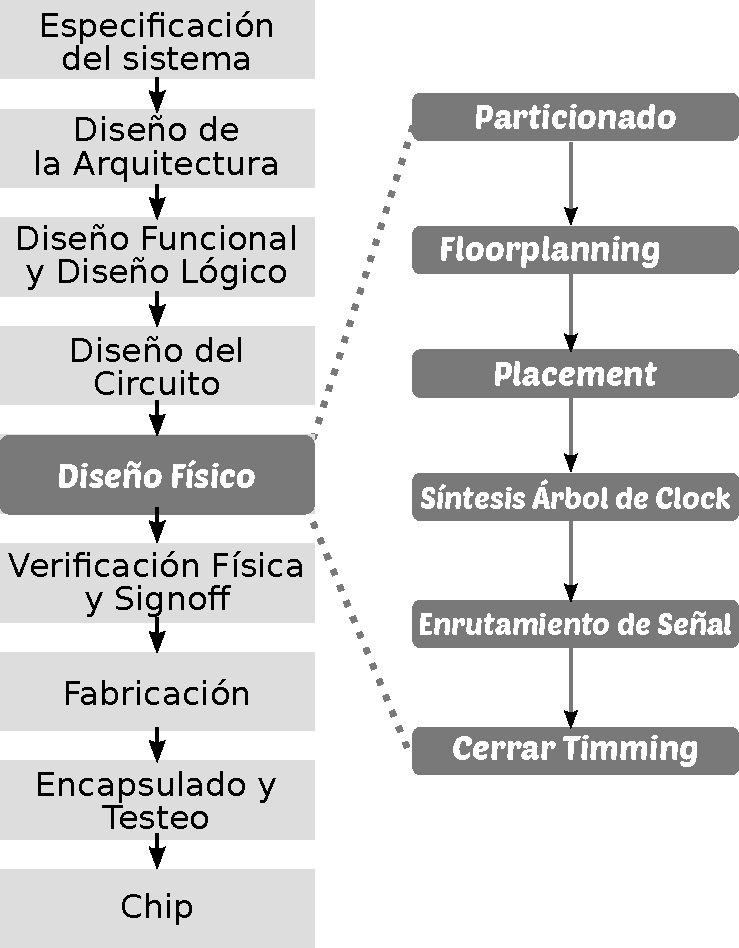
\includegraphics[scale=0.40]{figuras/DisenioFisico.pdf}
 \end{figure}

\end{frame}
%-------------------------------------------------------------
\section{Instalación y prueba}
\begin{frame}
  \frametitle{Instalación del flujo digital}
  Para instalar todas las herramientas, seguir las instrucciones detalladas en el repositorio que vamos a utilizar:

  \url{https://github.com/3ll34ndr0/dflow-doc}

  Asegurarse que todos los programas se hayan instalado correctamente.
\end{frame}
%-------------------------------------------------------------

\begin{frame}[fragile]
  \frametitle{Descargar los ejemplos y la configuración}
Descargamos todos los archivos de configuración para hacer funcionar todo el flujo con un diseño de prueba.

En un directorio cualquiera y desde la consola hacemos:
\begin{footnotesize}
  \begin{lstlisting}[language=bash]
git clone https://github.com/elleandroculia/dflow-doc.git
\end{lstlisting}
\end{footnotesize}

Probar el ejemplo:
\begin{footnotesize}
\begin{lstlisting}
cd ejemplos/test
qflow synthesize place buffer route display map9v3
\end{lstlisting}
\end{footnotesize}


El resultado final se mostrará en una ventana, donde podremos ver el circuito.

\end{frame}
%-------------------------------------------------------------

%-------------------------------------------------------------

\begin{frame}
\textbf{Flujo de diseño digital} 
   \begin{figure}[ht]
      \centering
      \scalebox{.14}{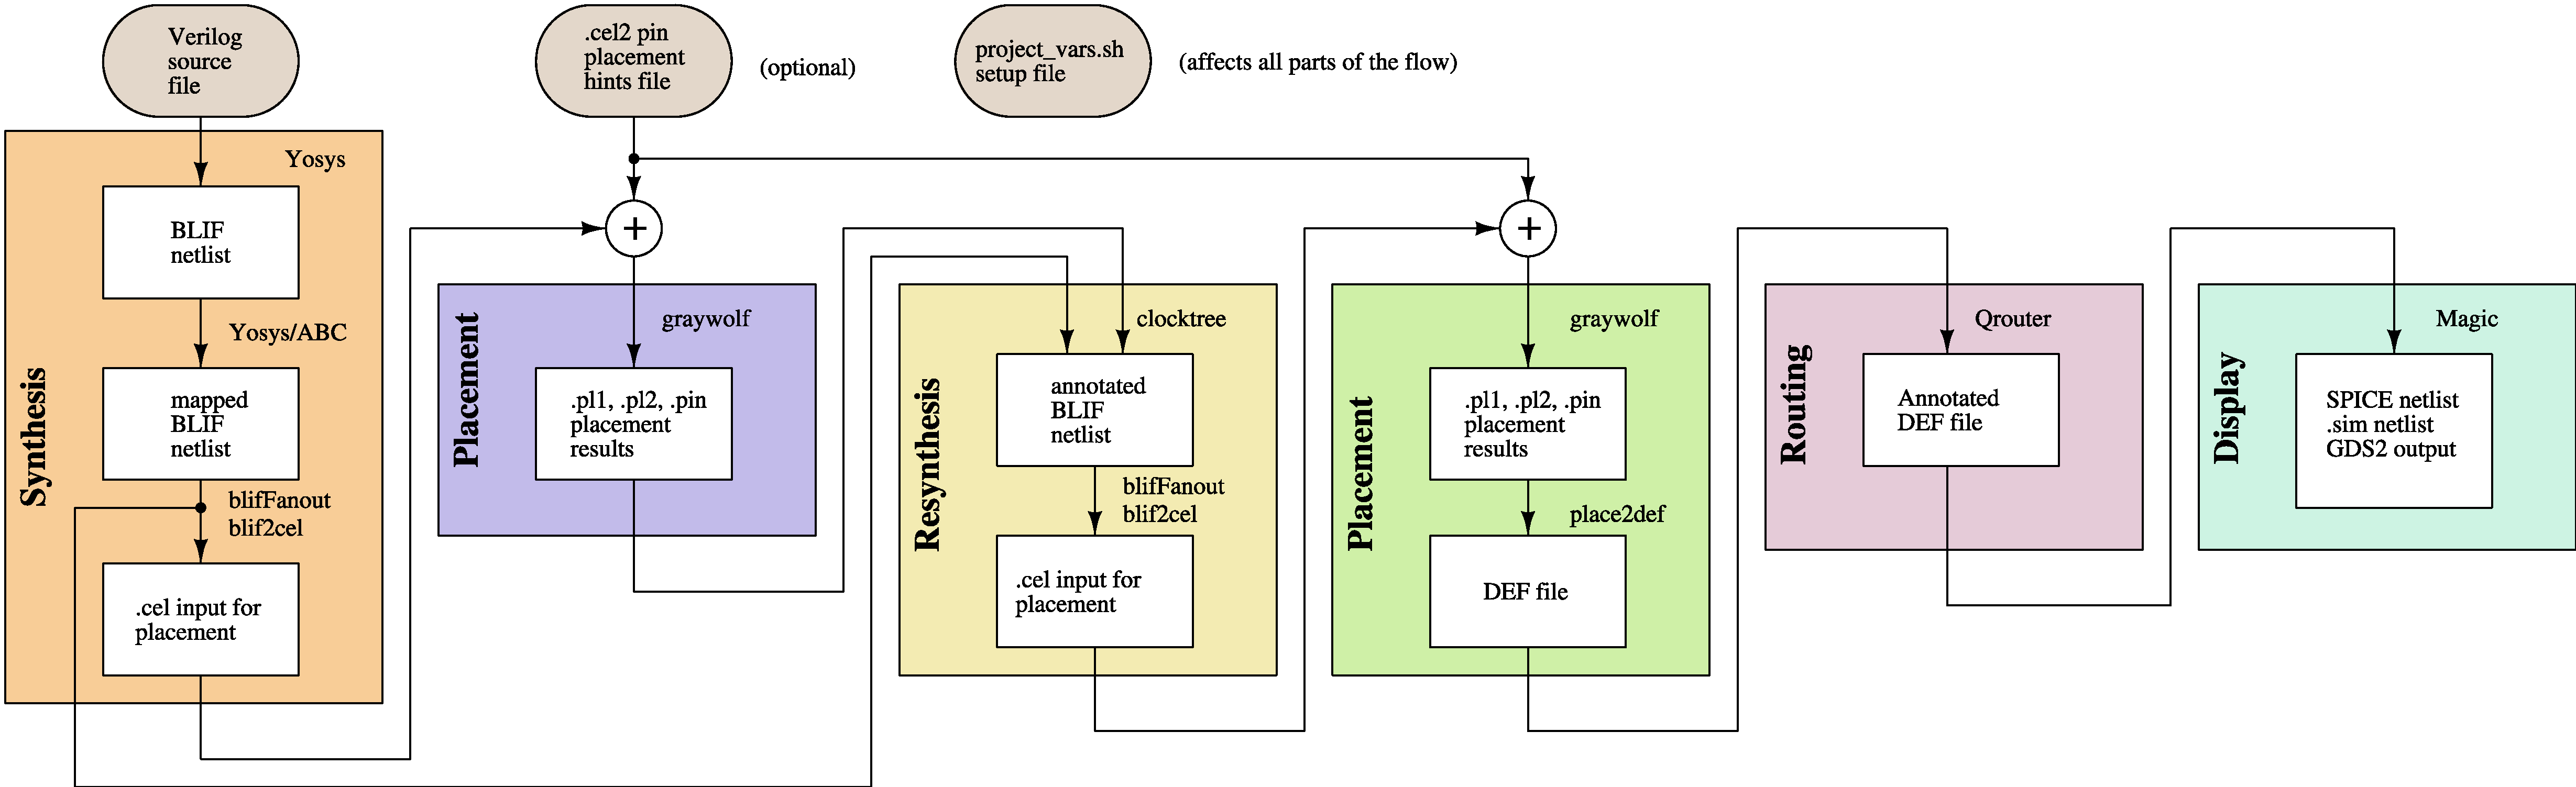
\includegraphics[angle=0]{figuras/qflow_the_flow.pdf}}
    \end{figure}
\end{frame}


%---------------------------------------------------
\begin{frame}
\frametitle{Design kit}
Por cada tecnología de fabricación, las herramientas necesitan un conjunto de archivos para cada etapa del diseño. Por ejemplo, archivo de configuración de DRC, un archivo con parámetros para hacer estimaciones de  \emph{timing} y potencia, librerías estándar, etc.

Nuestra herramienta trae instalada 2 design kits: OSU035 y OSU05


\end{frame}
%----------------------------------------------------
\begin{frame}[fragile]
  \frametitle{\emph{Síntesis de RTL a compuertas}}
  \textbf{Qflow} utiliza la herramienta \textbf{yosys} para generar un netlist verilog con sólo celdas estándar instanciadas, que funcionalmente sea equivalente al descripto a nivel de RTL.

  Qflow genera un script para síntesis completo en \verb.source./\emph{nombreDelModulo}.\textbf{ys}. Para modificarlo, copiarlo y cambiarle el nombre y en el archivo \emph{project\_vars.sh} poner la opción \textbf{yosys\_options} a "-s \emph{nuevoScript}.\textbf{ys}".

 
\end{frame}
%---------------------------------------------------

\begin{frame}[fragile]
  \frametitle{\emph{Floorplan y placement} con \textbf{graywolf}}
  \begin{exampleblock}{Herramienta de \emph{placement}}
    En \textbf{Qflow} se utiliza \textbf{graywolf}. El resultado que produce esta herramienta es un \emph{layout} en formato DEF, que representa al circuito realizado con celdas estándar instanciadas en el plano y los pines de entrada y salida.
  \end{exampleblock}
\end{frame}

\begin{frame}[fragile]
  \frametitle{Archivos para guiar la herramienta}

Para guiar el resultado de la herramienta, editar los archivos:
\begin{itemize}
  \item \emph{nombreDelMódulo}\verb#.cel# 
  \item \emph{nombreDelMódulo}\verb#.cel2# 
  \item \emph{nombreDelMódulo}\verb#.par#.
\end{itemize}

Por ejemplo, luego de la primera prueba podemos encontrar el archivo \verb#map9v3.par# en el directorio \verb.layout.:
\begin{exampleblock}{Modificar la cantidad de filas del floorplan}
Si descomentamos la línea:

\verb.#  GENR*numrows           : 6. 

nuestro \emph{floorplan} tendrá 6 filas de celdas. 
\end{exampleblock}
%  Se pueden indicar varios \emph{constraints} a esta herramienta: ubicación de los pines, cantidad de filas a utilizar, celdas de relleno, etc.

%    Para ubicar los pines de entrada y salida, editar el archivo ubicado en \verb.layout. con extención \verb.cel..  Con el archivo de extensión \verb.par. podemos indicar cantidad de filas de celdas estándar que serán usadas. Si no indicamos nada, graywolf intentará un \emph{floorplan} cuadrado.

\end{frame}

%---------------------------------------------------
\begin{frame}
  Descargar la documentación completa de Timberwolf:
  \begin{tiny}
  \url{https://github.com/rubund/timberwolf/raw/master/doc/TimberWolf.pdf}
\end{tiny}

Aclaración: \textbf{Qflow} utiliza \textbf{graywolf} que es un fork de \textbf{Timberwolf 1.3}, del cual sólo usa las herramientas de \emph{floorplan} y \emph{placement}.
\end{frame}


\begin{frame}
\frametitle{DEF/LEF}

\textbf{DEF}: Desing Exchange Format \\
\textbf{LEF}: Library Exchange Format \\


El formato es el mismo para ambos, pero cuando se utiliza para describir un bloque, se llama DEF, y para una libreria de celdas estandars se denomina LEF.
Se puede encontrar un archivo .lef con las reglas y definiciones de la tecnolog\'ia, y otro .lef con la librer\'ia de celdas est\'andar.\\
Este formato es lo que usa el ruteador y el placer (entre otras herramientas) para conocer aspectos fisicos de las celdas y los bloques. Tiene informaci\'on del layout y de la tecnolog\'ia. 



\end{frame}

%------------------------------------------------

\begin{frame}
\frametitle{DEF/LEF}
DEF: Desing Exchange Format \\
LEF: Library Exchange Format \\

\begin{center}¿Qué datos nos brinda este formato?
\end{center}
    \begin{itemize}
    \item Informaci\'on sobre DRC \'util para el ruteador, por ejemplo la separación mínima entre cables, m\'aximo ancho de pista, capas de obstrucción, Antenna Rules.
    \item B\'asicamente es informaci\'on de layout mas alguna informaci\'on extra \'util para el ruteador. Orientaci\'on de la celda o macrocelda.  
    \end{itemize}
\end{frame}

%----------------------------------------------------------------------------------------
\begin{frame}
  \frametitle{Modelos de timing y potencia} 

\textbf{NLDM: Non-Linear Delay Model} 

Es una forma de expresar los Delay, Timing Checks y Output Slew (tiempo de transici\'on) de bloques. Asume carga capacitiva pura, utilizando capacidad equivalente en el caso de que la resistencia no es despreciable. 

Para guardar esta información de las celdas, se utiliza el formato \textbf{Liberty}. Pero también se puede usar para caracterizar en tiempo y potencia bloques mas grandes, y poder usarlos como una caja negra.
\end{frame}

%------------------------------------------------
\begin{frame}[fragile]
  \frametitle{ Archivo .lib (Liberty)  }
  \begin{itemize}
    \item El archivo .lib contiene información de timing y potencia de todas las celdas estándars, y también puede incluir la función de la celda, entre otras propiedades. 

    \item Es un estandar abierto y suele venir incluido con la librería de celdas estándar.

    \item Es utilizado por la herramienta de síntesis \textbf{yosys} y la herramienta de STA (Static Timing Analisys) \textbf{vesta}
  \end{itemize}
\end{frame}
%-------------------------------------------------------------
\begin{frame}
\textbf{Formato y significado del archivo .lib} 
   \begin{figure}[ht]
      \centering
      \scalebox{.30}{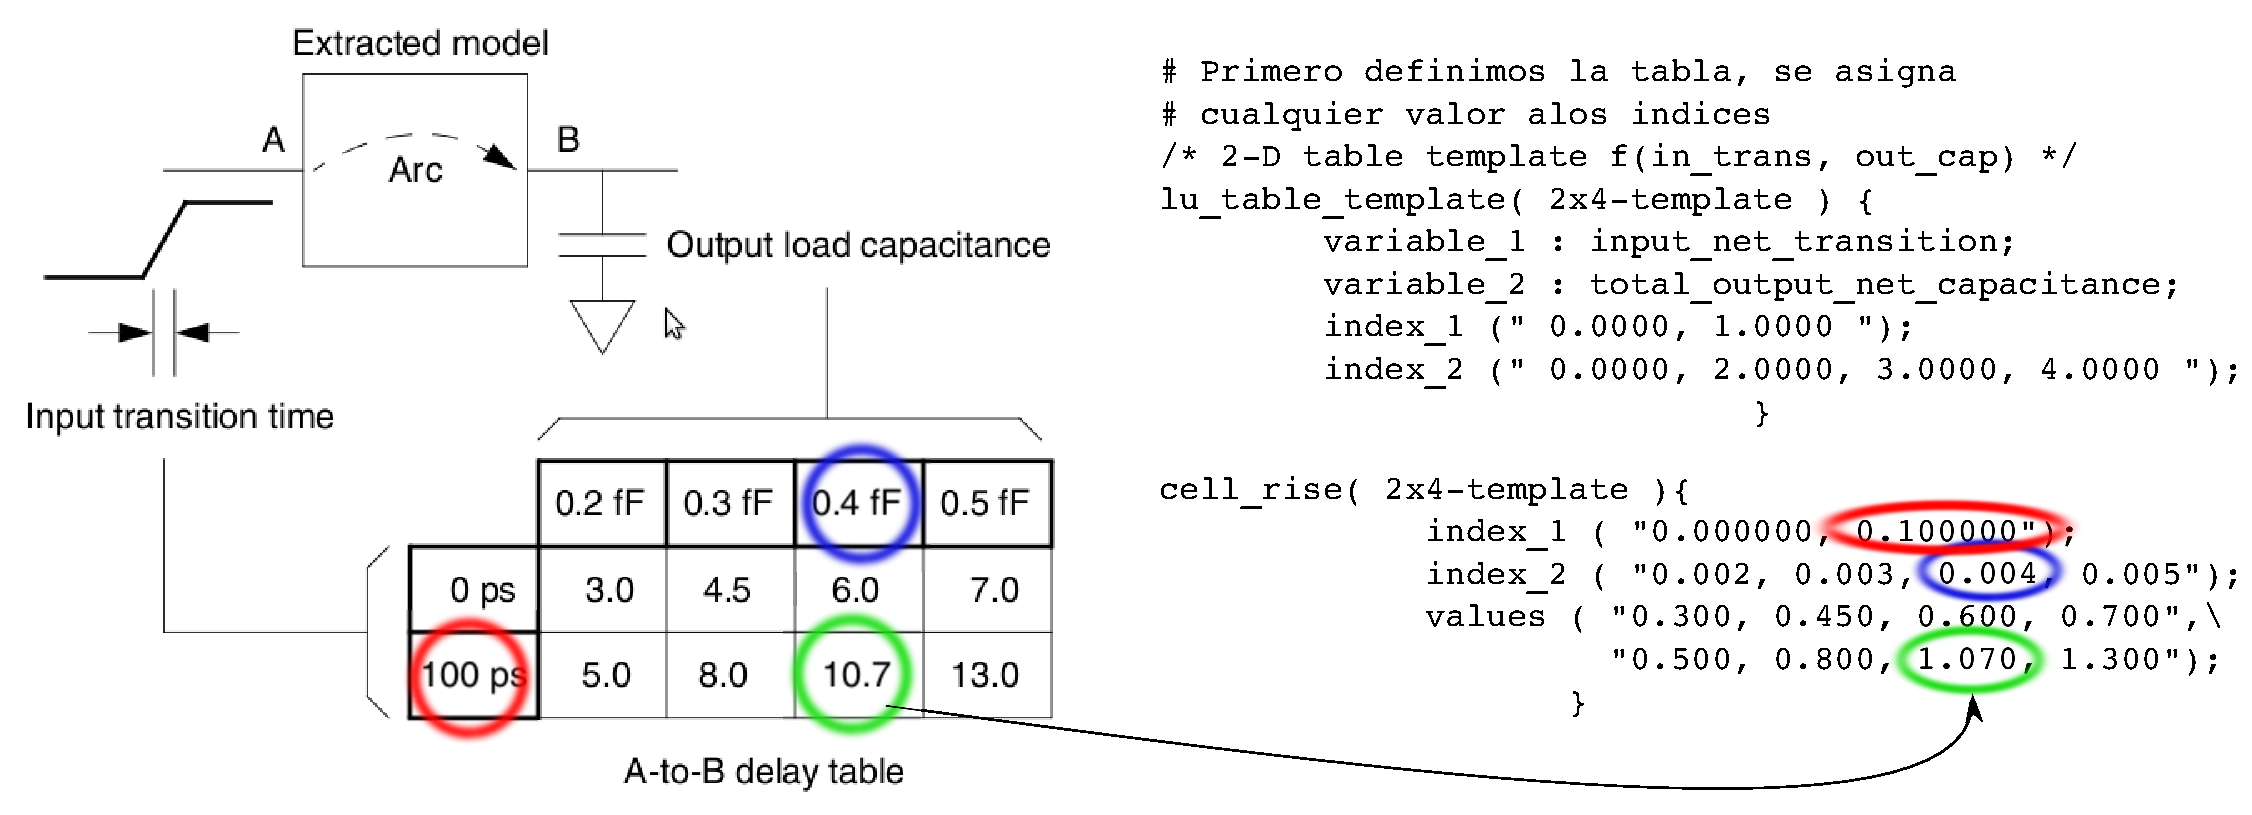
\includegraphics[angle=0]{figuras/delay-table.eps}}
    \end{figure}
\end{frame}


%----------------------------------------------------------------------------------------
%------------------------------------------------
\begin{frame}
  \begin{figure}[ht]
      \centering
      \scalebox{.65}{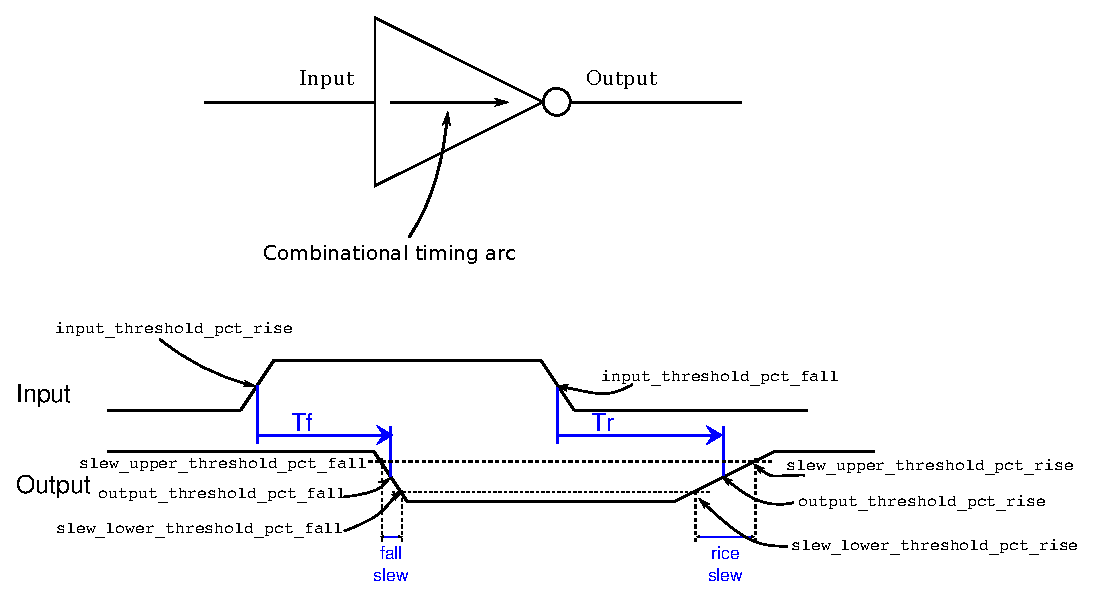
\includegraphics[angle=0]{figuras/inout-timing.eps}}
    \end{figure}
  
\end{frame}

%----------------------------------------------------
\begin{frame}
  \frametitle{Modelos de timing y potencia} 

 \textbf{NLDM: Non-Linear Delay Model} 
   \begin{figure}[ht]
      \centering
      \scalebox{.30}{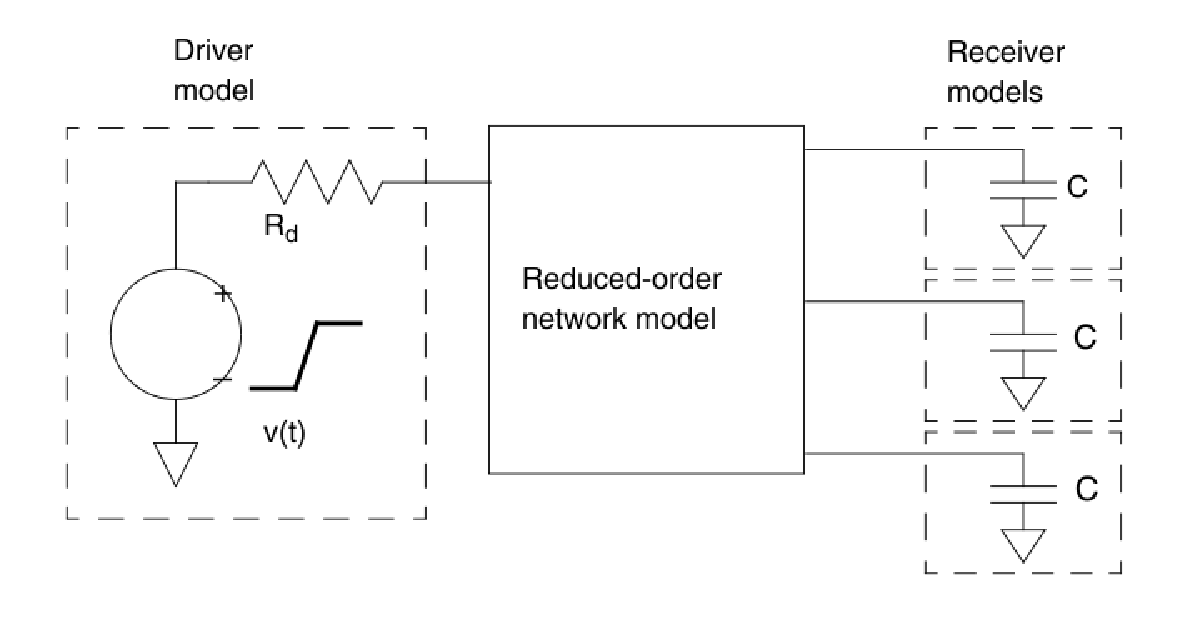
\includegraphics[angle=0]{figuras/nldm-model.eps}}
    \end{figure}
    Se especifica los tiempos según una tabla de 2 entradas:
    \begin{itemize}
	\item El tiempo de transición de la fuente de tensión a la entrada (driver)
	\item Capacidad de carga a la salida (receptor)
\end{itemize}

\end{frame}
%----------------------------------------------------------------------------------------

\begin{frame}[fragile]
  \frametitle{Ruteador}
  \textbf{Qflow} utiliza el ruteador \textbf{qrouter}

  En el archivo de configuración \verb#project_vars.sh# encontramos dos variables que influyen en el comportamiento del ruteador: \textbf{qrouter\_options}, \textbf{via\_stacks} y \textbf{via\_patterns}

  Otras opción importante es la de especificar los metales permitidos para rutear.
\end{frame}

%--------------------------------------------------------------------

\begin{frame}
\Huge{\centerline{Fin}}
\end{frame}

%----------------------------------------------------------------------------------------

\end{document} 
